\chapter{Technology Review}
In this chapter, I will be taking a look at all the technologies used to make up the final version of the project. I will be discussing what each of the technologies used for images, coding and games development are and what each of their purpose is in the project. For this, I will be going over why I used each of the technologies along with discussing the similar versions of them and why I chose not to use these other versions.

\section{Game Engines}
In this section I will be discussing each of the game engines I at before I decided on which one I was going to use. These include the Unity Game engine and the Unreal Engine 4. I will be discussing their features as well as why I thought they would be a good or bad engine to use for the project in terms of did they have the features that I required to meet my objectives and how user friendly they were to those ranging from beginners to those who are experts in the field of games development.\cite{GameEngines}
\newpage
\subsection{Unity Engine}
\begin{figure}[h]
  
\includegraphics[width=\linewidth]{Images/UnityLogo.png}
  \caption{Unity.}
  \label{fig:Unity}
\end{figure}
\bigskip


Unity is a cross-platform game engine which was first announced and released for free in June of 2005 at Apple Inc.'s Worldwide Developers Conference as a Mac-OS X exclusive game engine, which later became available for other systems like windows. As it is cross-platform, this means that any game you make in it can be played on any console or computer such as the Xbox One, PlayStation 4, Windows OS, Linux OS and Android. The engine can produce 3-Dimensional as well as 2-Dimensional games, Virtual Reality Games and Augmented Reality Games and mainly uses the C\# scripting language. During the last 2 years of the Software Development course, this engine was used to teach us Mobile App Development where we developed games on it. I have used this engine to create 3D and 2D games from both what I have been thought in class as well as using Unity's own online lessons which release on the regular when ever a new version of the software comes out. However, even if what you want to learn how to do is not available on the lessons section on their website yet, there are hundreds of YouTube tutorials out there from the massive community of people who use this engine. 
Unity also comes with its own asset store which people can put up on the asset store for free or for a small or large fee. The assets can be anything form 3D or 2D character or level designs, level and game music and also packages like Text Mesh Pro which makes a more crisp looking text than the one that Unity has as a default, which I will touch on more later on.
Unity also has an impressive library of games made using their engine such as the multi-award winning title "Ori and The Blind Forest" which is a 3D sidescroller adventure game and which has since produced a sequel titled "Ori and the Will of the Wisps" in which it has done equally as well as its predecessor.\cite{Unity}
\newpage

\subsection{Unreal Engine(UE4)}
\begin{figure}[h]
  
\includegraphics[width=\linewidth]{Images/Unreal-Engine-Logo.png}
  \caption{Unreal.}
  \label{fig:Unreal}
\end{figure}
\bigskip

Unreal Engine is a game engine developed by Epic Games, who in recent times has become well known due to their release of the popular battle royal title "Fortnite". It was first showcased in 1998 to be used in development for FPS(First-Person Shooter) games, but has since been used successfully in genres like platformers, fighting games and other RPGS(Role-Playing games). The current version, Unreal Engine 4, was originally released in 2014 as a subscriptions service with the first game released being a 3D Horror game Called "Daylight" but later became free to download the following year with its source code being available on GitHub. Unreal Engine uses the C++ language to develop its games. Similar to the Unity engine Unreal offers its own asset store, the Unreal Engine Marketplace, where users can buy art, character models, sounds and environments to name a few, along with tutorials and other guides on how to make your desired game.
Although it is possible to make 2D games on the Unreal Engine 4 with the project set up for 2D side-scroller now available, it was originally designed for it's main clear focus  on that of 3D graphics and shaders. To take "Bloodstained: Ritual of the Night" as an example of the capabilities of Unreal Engine 4s 2D development as you can see from figure \ref{fig:Bloodstained} that it has 3D models working on a 2D landscape.\cite{UnrealEngine4}

\begin{figure}[h]
  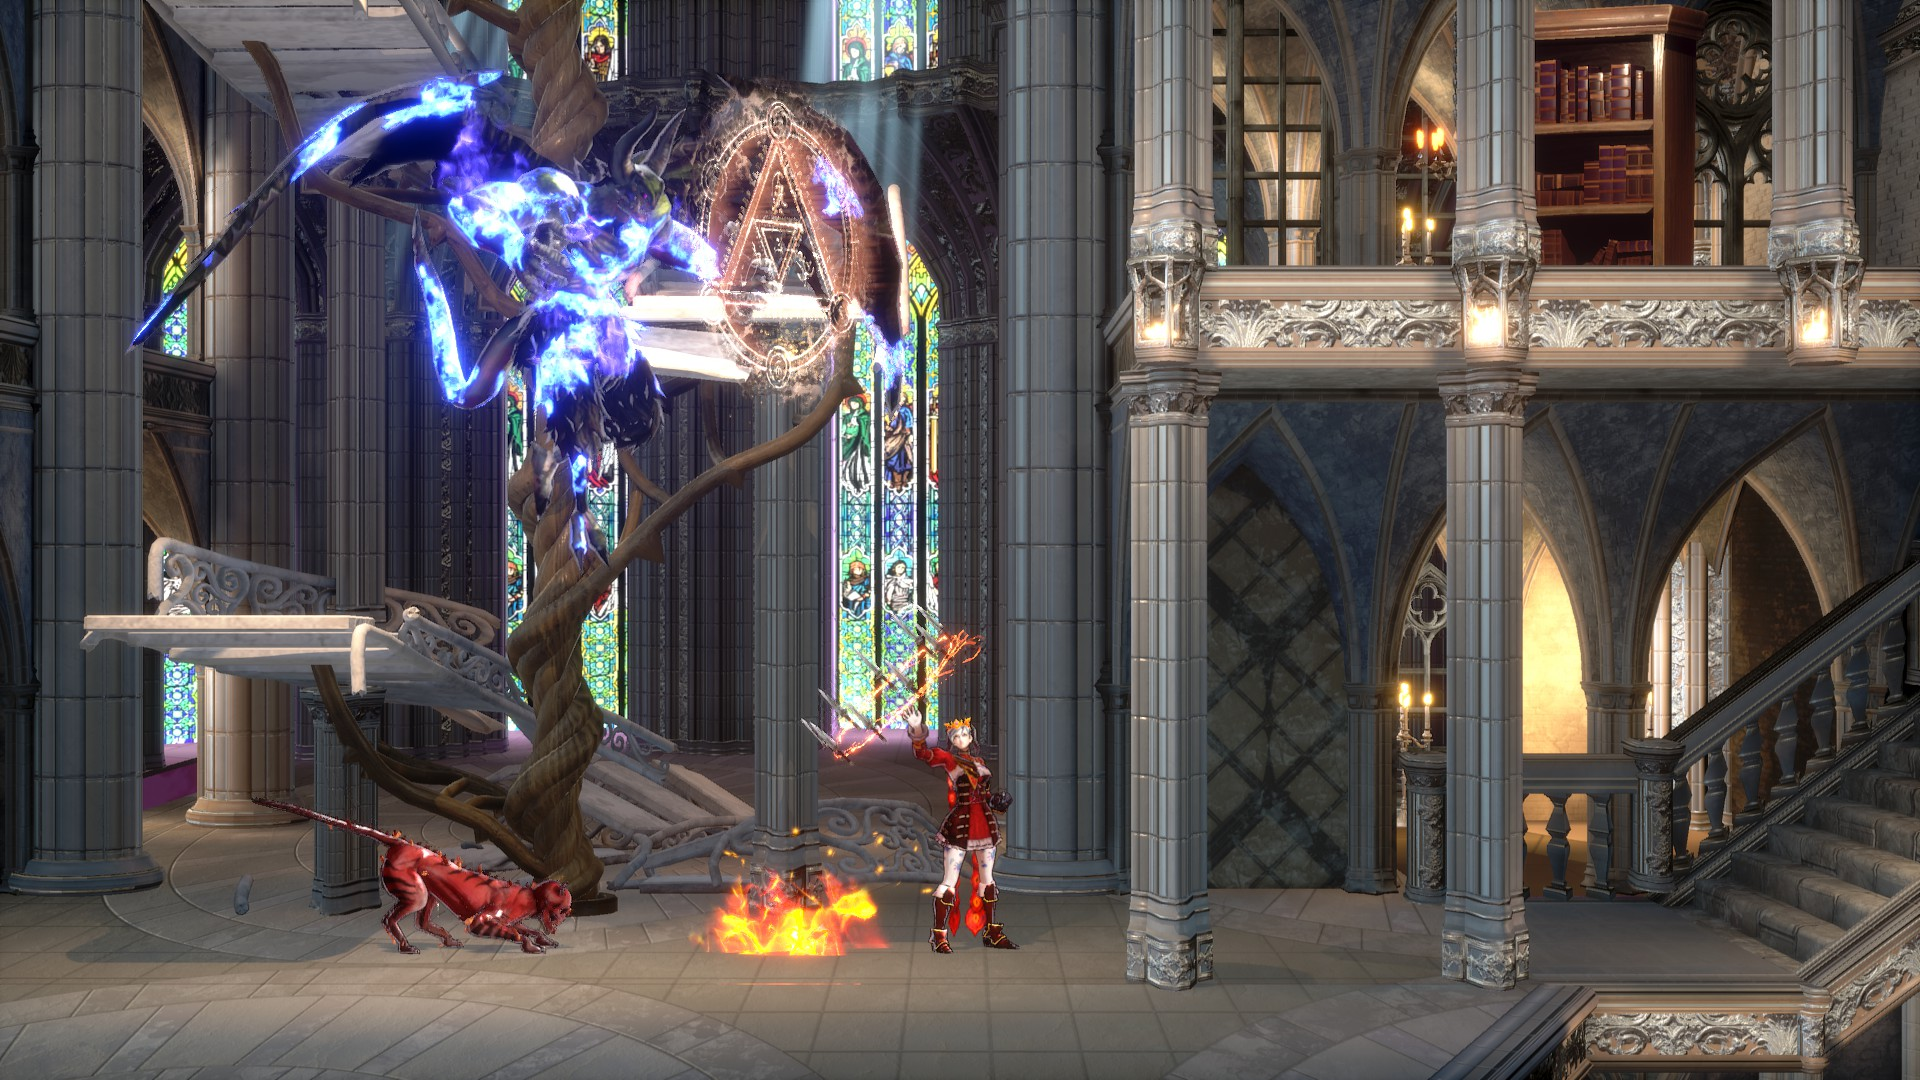
\includegraphics[width=\linewidth]{Images/Bloodstained-1080.jpg}
  \caption{Bloodstained.}
  \label{fig:Bloodstained}
\end{figure}

\newpage
\subsection{Unity Engine or Unreal Engine 4?}
\begin{figure}[h]
  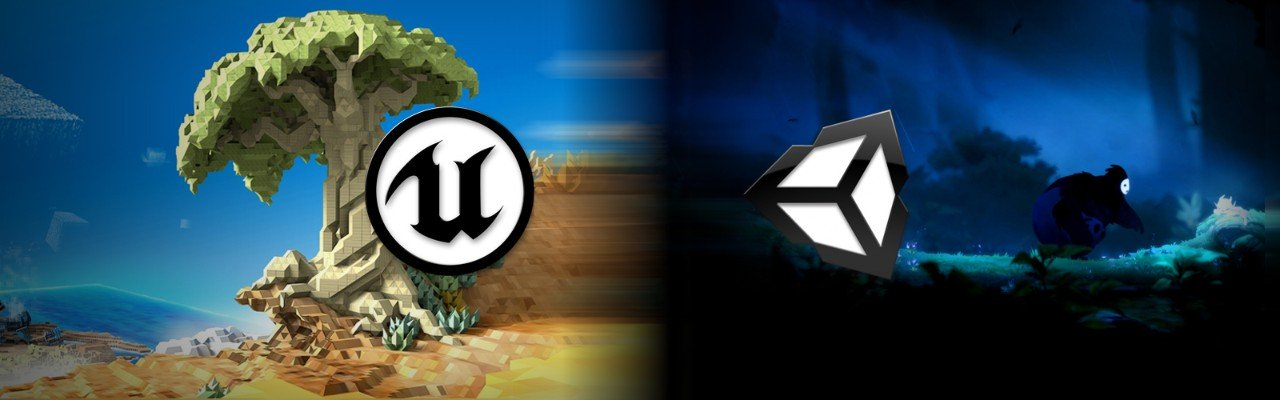
\includegraphics[width=\linewidth]{Images/UnrealVSUnity.jpg}
  \caption{Unreal vs Unity.}
  \label{fig:Unreal vs Unity}
\end{figure}
\bigskip

For this project, I had an early mindset that I wanted to create a 2-Dimensional game as I find it is a lot easier for people, myself included, that are not exactly the best artists or designers to create something that looks visually decent compared to having to learn how to use 3d modeling software's like Blender, which is used for creating 3d models, in order to create the level design and the character design. In order for me to use the Unreal Engine, I felt that after researching on it I came to the conclusion that it would not meet my requirements in order to create a 2D game as although it is possible to make a 2D game, it is mainly used for the creation of 3D games. Unreal Engine is also an engine that offers very high visuals, which means that it is much more suited to make a high end games more suited to big games development companies over a single person making a game.
Unity is more widely used for small teams or a single person making a small to medium scale games, although it is possible to make a high end large scale game, it is more suited to the small teams or singular developers. As well as this, Unity for me seemed much more user friendly as when you click to start a new project, it will give you an option to start a new 2D project and will take it as you are using 2D features for the build. I felt as though it was easier to find exactly what I was looking for when I searched online or on YouTube for ways to do certain things related to 2D development than searching for how to do it on the Unreal Engine as there was a lot of examples out there and even Unity's forum was full of guides and lessons on how to add features such as 2D level designing, background layer designs and enemy AI tracking to name a few.
To conclude, Unity was the game engine I went for, not only because I felt it met my requirements for making a 2D game, but because of the fact Unity mainly uses C\# as its main language over Unreal 4's C++ language. This is not to say that the C\# is better than the C++ language, but I felt that as I have gained experience in using the C\# language through modules in the Software development course that it would be better for me to expand on what I already knew and what I found that I have an interest in. I also chose Unity because since I first used it back in my second year for a project where I made a short shooter game, I found it very user friendly and relatively easy to learn all of its features through its online learning course and found the C\# language easier and more interesting to learn for me compared to other languages like Java, C++, HTML, etc.\cite{UnityVUnreal}

\newpage

\section{Packages}
The following section will discuss the packages used in unity for the development of the game. Packages are collections of files and data from Unity projects, or elements of projects, which are compressed and stored in one file, similar to Zip files. Like Zip files, a package maintains its original directory structure when it is unpacked, as well as meta-data about assets (such as import settings and links to other assets). For my project I used the packages TextMesh Pro for the use of text in my UI.\cite{UnityPackages}

\subsection{TextMeshPro}
The TextMesh Pro package in Unity is used as a replacement for Unity's standard UI Text and Text Mesh. It uses advanced Text Rendering and custom text shaders which allows for visual quality improvements in the text while also allowing users to put there own style of text styling and texturing. It can also enable users more control over text formatting and layout features such as word, line and paragraph spacing.\cite{TMPRO}

\begin{figure}[h]
  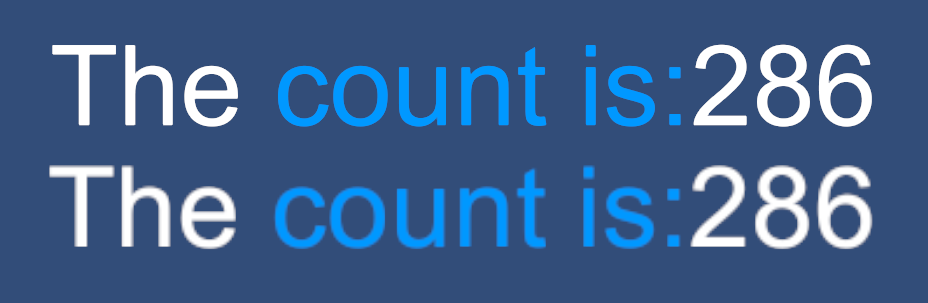
\includegraphics[width=\linewidth]{Images/TMProTopvStandardBottom.PNG}
  \caption{TMP Pro(Top) vs Standard Text(Bottom).}
  \label{fig:TMP V Text}
\end{figure}




\section{Sprite Editors/Creators}

In this section I will be going through which image creation software I used in order to create the sprites that I needed for my character designs, level design and other general things like health items or collectables. For this, I looked into different Image editors like Inkscape, Krita, Adobe Photoshop and Gimp and decided to narrow it down to Gimp and Photoshop as I have had past experience in both of them. I will discuss both in terms of how user friendly they are and did they meet the requirements that I needed in order to create the art sprites for my game also taking into to consideration that drawing would not be my strong point.
\newpage

\subsection{Gimp}
\begin{figure}[h]
  
\includegraphics[width=\linewidth]{Images/gimp-logo.png}
  \caption{Gimp.}
  \label{fig:Gimp}
\end{figure}
Gimp(GNU Image Manipulation Program) is a open-source raster graphics editor that can be downloaded for free online. It is has many capabilities such as a photo retouching program, a online batch processing system, a image format converter and it can be used as a simple paint program to name just a few of its features. It's first version was released in back in 1996 being ported to windows operating system in 1997. GIMP is considered a good alternative to Adobe Photoshop as it is a free to use software with no subscription fee. In terms of video game development, GIMP is plenty powerful enough to support art for games as it was used to create nearly all the artwork for "Lucas the Game" which was made back in 2014 with the developer Timothy Courtney stating, "GIMP is a powerful tool, fully capable of large professional projects, such as video games."
GIMP is also capable of producing animations by using it's GIMP Animation Package(GAP) which is a plug-in for creating animations on the software. It can save and export animations in several formats including the most popular and widely used GIF and AVI formats. The GIMP website also offers plenty of tutorials available through its website where it teaches beginners how to start using the software, how to edit photo's such as converting to black and white, tone mapping with colours and exposure, painting tutorials and programming tutorials to name a few. It also has a long list of video tutorials available on YouTube ranging from beginners to experts.
Overall GIMP is a very user friendly image editing software that is only made better by the fact that it is free to use.\cite{GIMP},\cite{GIMPTutorial}
\newpage

\subsection{Adobe Photoshop}
\begin{figure}[h]
  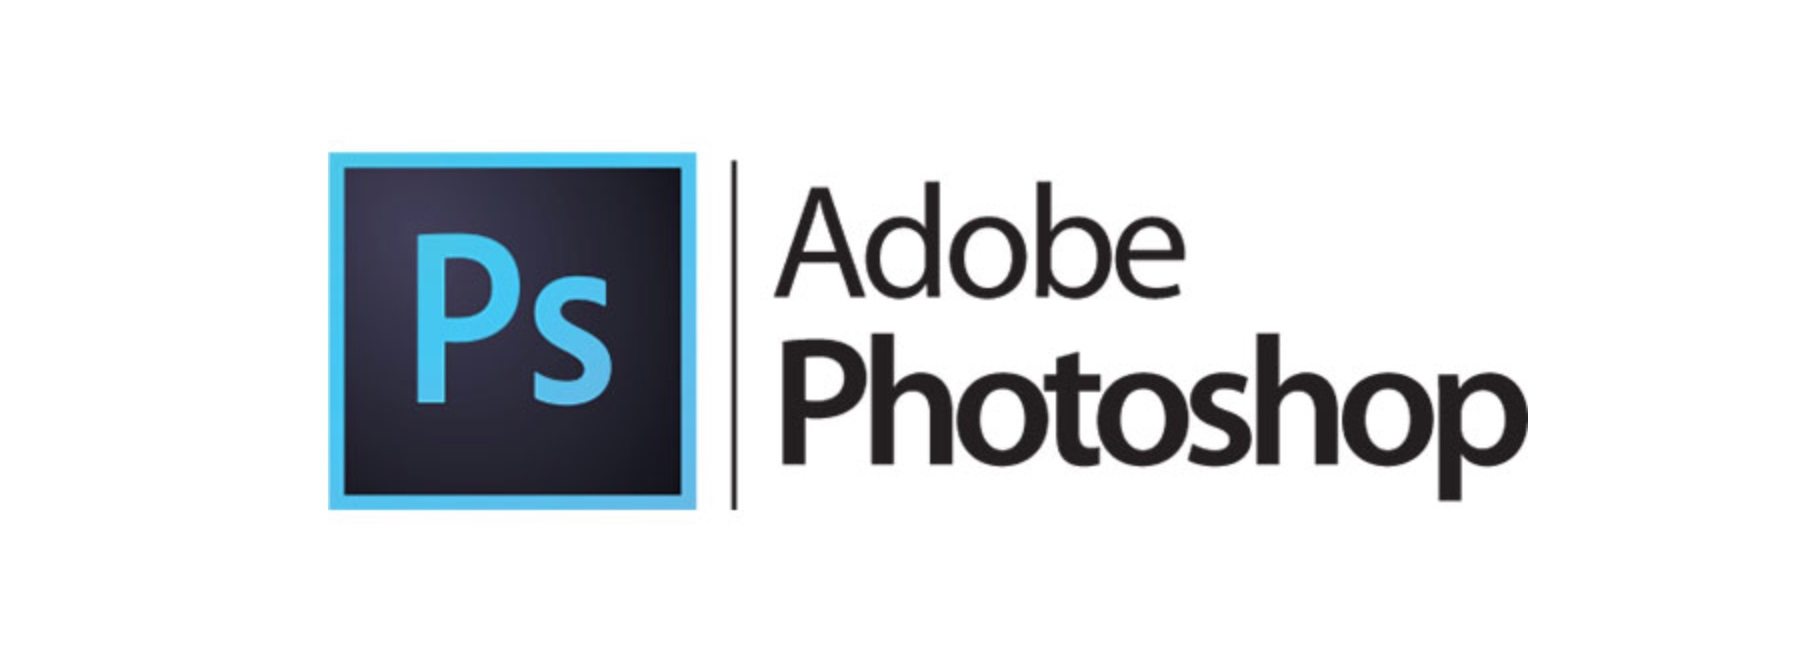
\includegraphics[width=\linewidth]{Images/adobe-photoshop.jpg}
  \caption{Adobe Photoshop.}
  \label{fig:Photoshop}
\end{figure}
Adobe Photoshop is a raster graphics editor developed and published by Adobe Inc. that was released in April of 1990. The software has become an industry standard for raster graphics editing and digital art. It is widely used by those in games development to produce the art for the games. Photoshop can compose and edit photos using multiple layers and several colour models such as RGB and duotone. Photoshop also boasts its own file formats, PSD and PSB, to support those features. A PSD(Photoshop Document) file contains a maximum of thirty thousand pixels for width and height while also allowing for a file length limit of 2 gigabytes, which is plenty big for just about any project. The other file format, PSB(Photoshop Big), is a larger version of the PSD format as it extends the pixels allowed to 300,000 pixels and extends the file limit to 4 exabytes, which totals to a massive 4000 gigabytes. Photoshop offers plenty in terms of video editing using video file formats such as MOV and MPEG-4 as well as capabilities to transform 2D elements of artwork to easily become 3D with a click of a button. Photoshop has reached such a height of popularity that it has even become a verb, as most people who see an image that has clearly been edited would state "That image has been Photoshopped" instead of simply saying it's been edited.
The Adobe website offers plenty of tutorials to both beginners and those who are experienced by being able to separate into beginner lessons, where you learn the basics like getting to now Photoshop, and experienced lessons like how to work on Photoshop using a tablet such as an iPad. Even if there is something that cant be found through their website, there are hundreds of tutorials available online and through YouTube.
Photoshop is not free however, as it charges a monthly subscription in order to use its services ranging from  \EUR{12.29} per month to  \EUR{24.59} per month. There is currently a cheaper price available to students and teachers of \EUR{19.99} per month.\cite{AdobePhotoshop}\cite{AboutAdobePhotoshop}

\subsection{Gimp or Adobe Photoshop?}


As I have stated previously, I wanted to create a simple 2D design type of game which would not require a lot of skill in terms of art and I took this into account while researching which image editor software to use. Early on I ruled out using Inkscape and Krita as even though they seemed like good tools, I had previous experience in both GIMP and Adobe Photoshop so I decided to stick to what I knew and work on further expanding my knowledge of what was familiar. Both Gimp and Photoshop are fantastic Image editor software's but the ultimate turning point on choosing one over the other came down to the price and my prior knowledge.
Due to this I decided to go with the free software GIMP over the subscription service of Photoshop. Although Photoshop is the more widely known software, the subscription fee turned me away from it as GIMP, being free, has more than enough tools in it for what I needed to make the artwork for my game. Along with this reasoning was the fact that I have used GIMP far more than I have used Photoshop so i wanted to stick to what I was more familiar with and further expand my knowledge on it for any future projects I intend to create in the future. For two of my previous projects in the software development course where developed a game, I used the GIMP software in order to create the artwork, this being another reason I was being pulled toward using GIMP. This is no in way saying that GIMP is a better software over Photoshop, as personally I think that Photoshop does seem to be the better software after researching and using both it and GIMP. However, for the purpose of making this game, I felt that GIMP was capable of providing me with exactly what I needed for the games artwork, without having to go paying for a subscription fee like Photoshop.\cite{AdobePhotoshopVGIMP},\cite{GIMP},\cite{AdobePhotoshop}
\begin{figure}[h]
  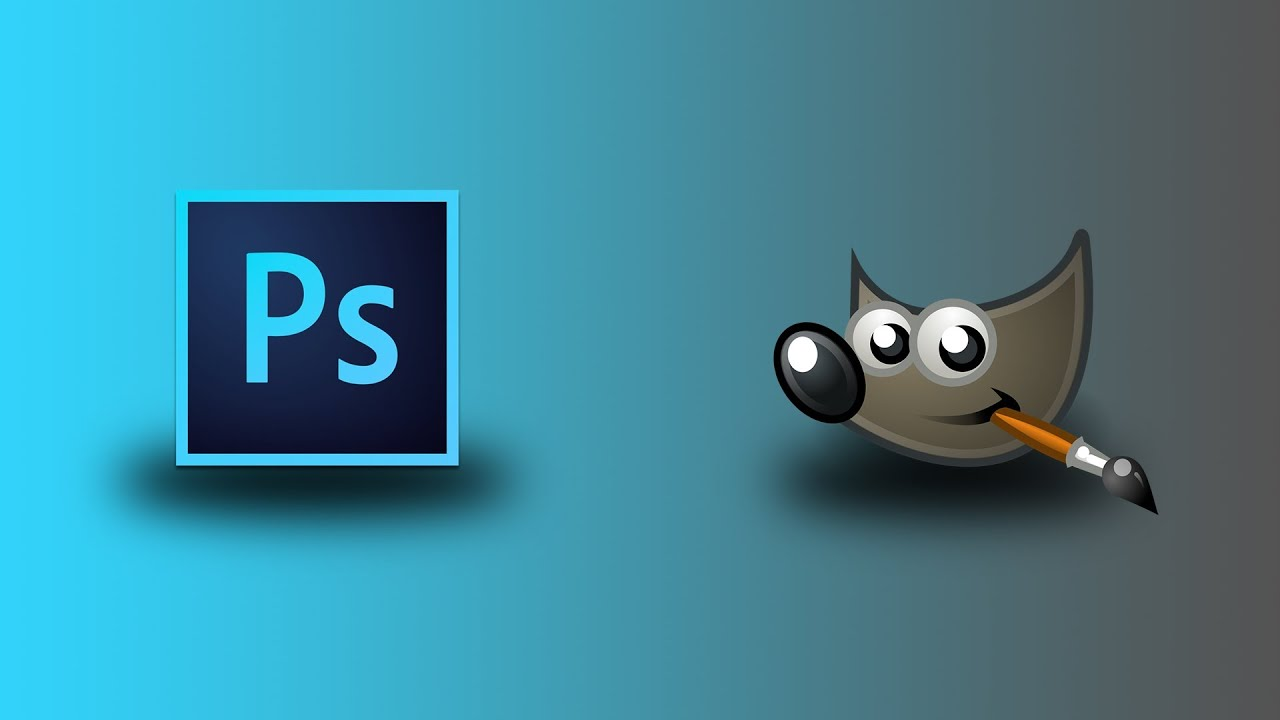
\includegraphics[width=\linewidth]{Images/GimpVphotoshop.jpg}
  \caption{Gimp vs Photoshop.}
  \label{fig:GimpVPhoto}
\end{figure}


\section{Languages}

\subsection{C Sharp (C\#)}

\begin{figure}[h]
  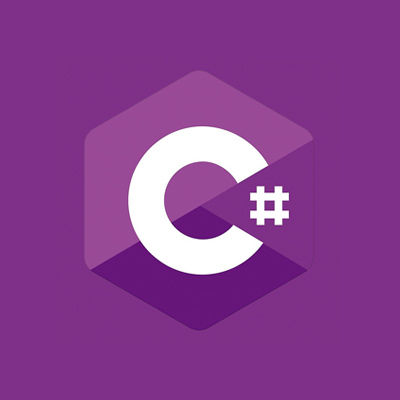
\includegraphics[scale=.5]{Images/C-sharp-logo.jpg}
  \caption{C\#.}
  \label{fig:C-Sharp}
\end{figure}

C\# is a general purpose, multi-paradigm programming language that has strong typing, functional, generic, object-oriented class based and component-oriented programming disciplines. Developed in 2000 by Microsoft, it is a programming language designed for the Common Language Infrastructure(CLI), which is an open specification developed by Microsoft. The C\# language is one of the main programming languages that is used in the development of a Unity project. Below is an example of a C\# script made for Unity.\cite{CSharp}
\begin{figure}[h]
  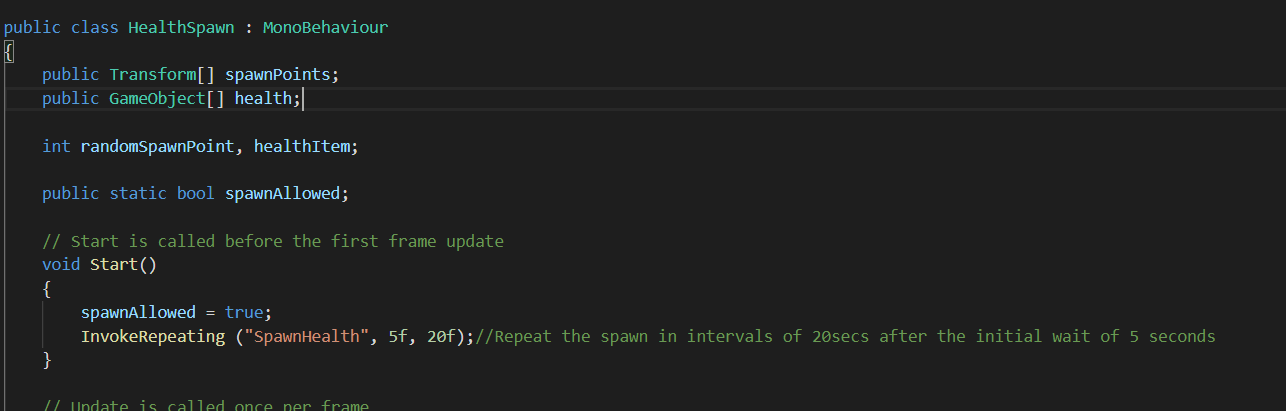
\includegraphics[width=\linewidth]{Images/C-Sharp-Example.PNG}
\newpage
  \label{fig:C-Sharp Example}
\end{figure}

\newpage
\subsection{\LaTeX}
\LaTeX \space is a text processor that is built around a markup language, which is similar to HTML.
Like HTML, \LaTeX \space uses tags to define a command or an action to display the text in a certain way. Tags are only seen in the source of the document will be hidden when the document gets compiled into the format of a PDF, see figure \ref{fig:LaTeXExample}
\begin{figure}[h]
  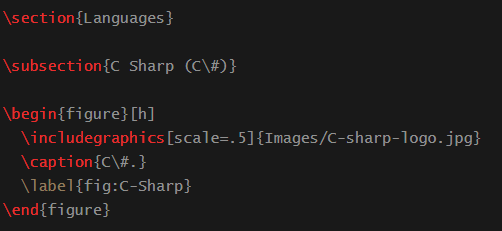
\includegraphics[width=\linewidth]{Images/Latex-example.PNG}
  \caption{LaTeX Example.}
  \label{fig:LaTeXExample}
\end{figure}
\bigskip
\newline
\LaTeX \space then compiles the text into a document like the PDF you are reading right now. It then renders the chapter, the section, the sub section and compiles it into the table of contents.\cite{LaTeX}

\newpage

\section{Other Software Used}
\subsection{Visual Studio Code}
Visual Studio Code is a source-code editor developed by Microsoft for Windows, Linux and MacOS. It comes with support for debugging, embedded Git control, syntax highlighting, intelligent code completion and code refactoring included. It has customizable features such as the editor's theme, preferences and keyboard shortcuts. The reason I used this was because it was exactly what I needed as Visual Studio Code offers specialized extensions that make developing with the C\# language much better.\cite{VSCode}, 
\begin{figure}[h]
  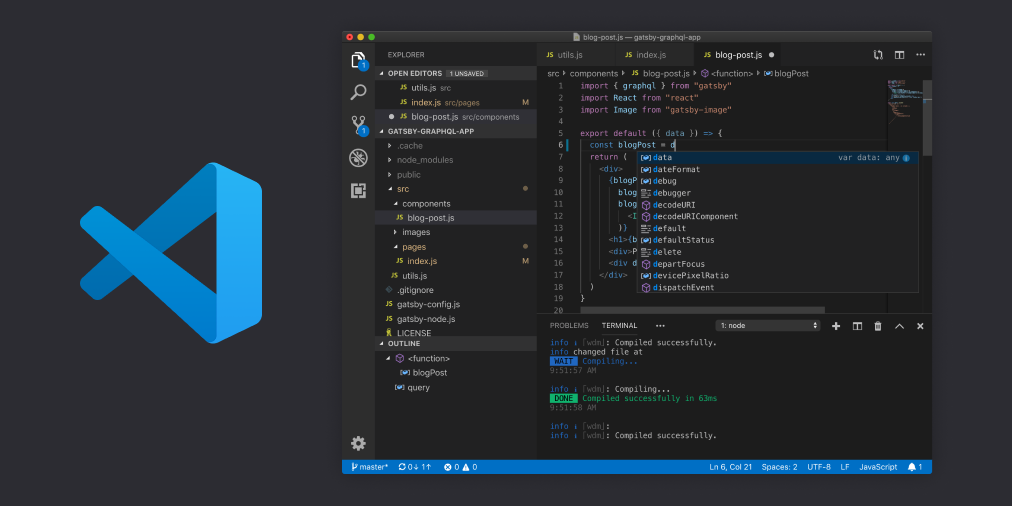
\includegraphics[width=\linewidth]{Images/VSCode.png}
  \caption{Visual Studio Code View.}
  \label{fig:VSCode}
\end{figure}